\documentclass{article}
%% PACKAGES %%

\usepackage{amsmath, amsfonts, amssymb, amsthm}
\usepackage{braket}
\usepackage{listings}
\usepackage{geometry}
\usepackage{xcolor}
\usepackage{textcomp}
\usepackage{graphicx}
\usepackage{fancyhdr}
\usepackage{sourcecodepro}
\usepackage{multirow}

%%%%%%%%%%%%%%

\graphicspath{{./images}}
\setlength\parindent{0pt}       % globally supress indentation

%% LISTINGS CONFIG %%

\definecolor{purple2}{RGB}{153,0,153} % there's actually no standard purple
\definecolor{green2}{RGB}{0,153,0} % a darker green

\lstset{
  language=MATLAB,                   % the language
  basicstyle=\normalsize\ttfamily,   % size of the fonts for the code
  frame = single,
  % Color settings to match IDLE style
  keywordstyle=\color{orange},       % core keywords
  keywordstyle={[2]\color{purple2}}, % built-ins
  stringstyle=\color{green2},%
  showstringspaces=false,
  commentstyle=\color{red},%
  upquote=true,                      % requires textcomp
  numbers=left,
  breaklines=true,
}

% Title Stuff
\title{\vspace{-3cm}ECE355L Project 3 \\ Part I: Convolution Calculations}
\author{Chase A. Lotito, \textit{SIUC Undergraduate}}
\date{}

\begin{document}

\pagestyle{fancy}

% attempt to make nice header
\fancyhead{}
\fancyhead[CH]{\normalsize{LOTITO --- ECE355L --- PROJECT 3, PART 1}}

\maketitle % Makes the title

\section*{Exercise 1}

Plot the respective graphs for the above examples and include in the report.

\smallskip

\textbf{Solution.}

\smallskip

All I did was copy the code from the lab manual, and after running those MATLAB scripts, I get the following plots:

\begin{figure}[!ht] 
    \centering
    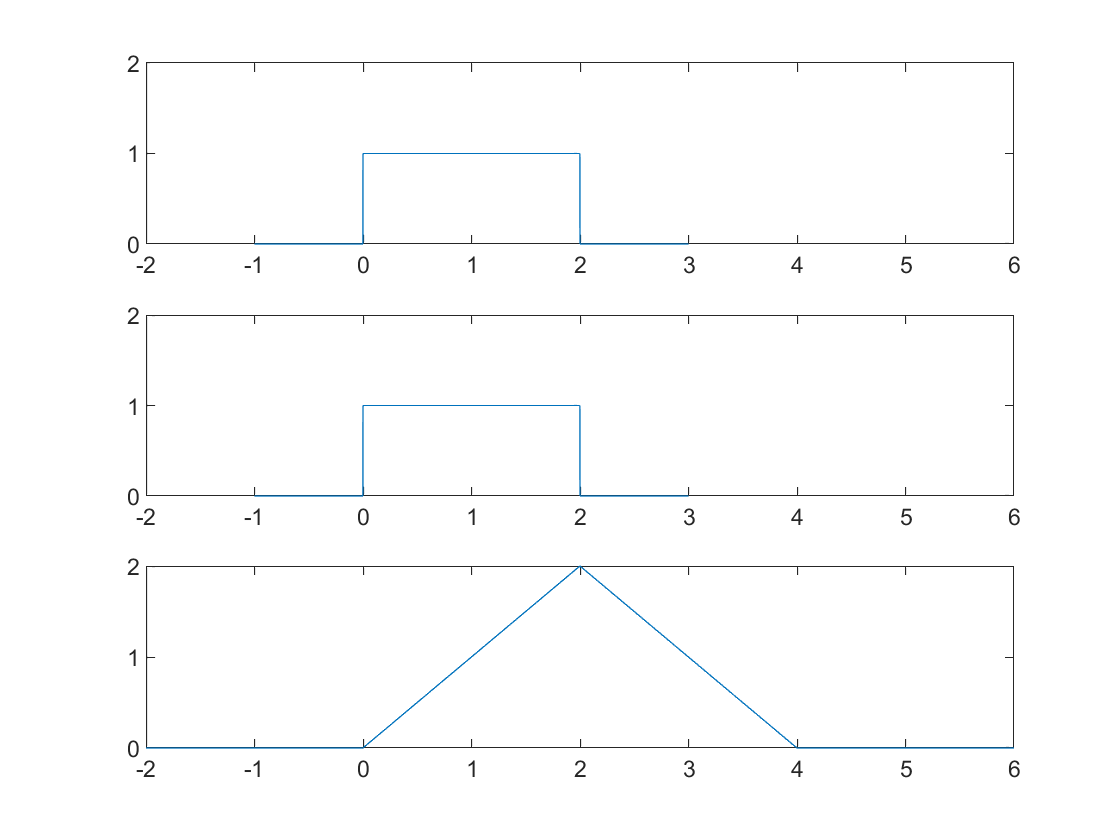
\includegraphics[width = 7cm]{plot1.png}
    \caption{Example 1 Plot}
    \label{fig:firstplot}
\end{figure}

\begin{figure}[!ht] 
    \centering
    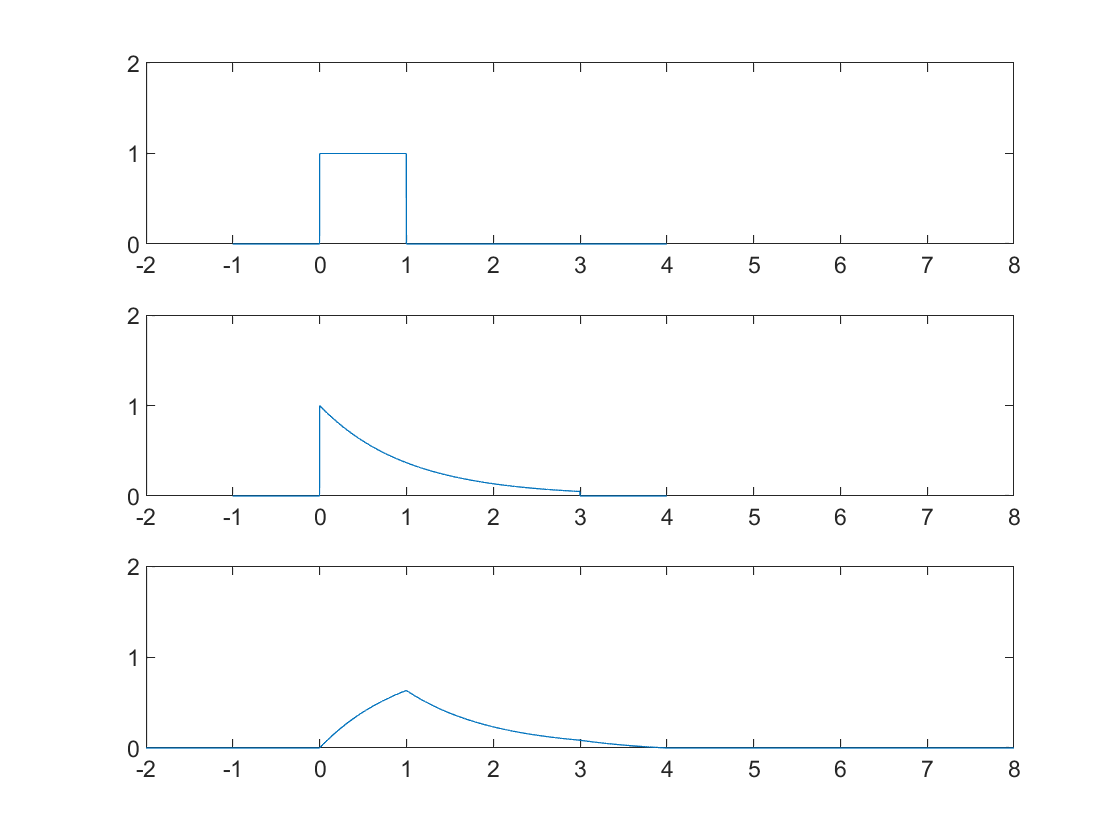
\includegraphics[width = 7cm]{plot2.png}
    \caption{Example 2 Plot}
    \label{fig:secondplot}
\end{figure}

\clearpage

\section*{Exercise 2}

Plot the following signals on the same window, but separate graphs using the subplot command and axis so that all graphs have the same range for the time (as was done in the examples). Let \(-2 \leq t \leq 25\) with a step size of 0.001 for \(f(t)\) and \(g(t)\). The convolution, \(y(t)\), product will then be evaluated for \(-4 \leq t \leq 50\).

\begin{equation*}
    \begin{gathered}
        f(t) = \sin \left( \frac{\pi}{10} t \right) \times [u(t) - u(t-20)] \\
        g(t) = \cos \left( \frac{\pi}{5} t \right) \times [u(t) - u(t-15)]  \\
        y(t) = f(t) * g(t)
    \end{gathered}
\end{equation*}

\smallskip

\textbf{Solution.}

\smallskip

To convolve \(f\) and \(g\) and then plot them with \(y\), I wrote the following MATLAB code:

\begin{lstlisting}
% Chase Lotito - ECE355L - Project 3
% PART 1: Plotting Convolutions
% Question 2

dt = 0.001;     % step size
t = -2:dt:25;   % f and g interval
t_y = -4:dt:50; % convolution interval

f = sin(t * pi / 10) .* rectpuls((t-10), 20);
g = cos(t * pi / 5) .* rectpuls((t-7.5), 15);
y = dt*conv(f, g);

% Plot all the convolutions
subplot(3,1,1), plot(t,f), title('f(t)'), axis([-2 25 -2 2]);
subplot(3,1,2), plot(t,g), title('g(t)'), axis([-2 25 -2 2]);
subplot(3,1,3), plot(t_y,y, 'r'), title('y(t) = f(t) * g(t)'), axis([-4 50 -3 2]);
\end{lstlisting}

The output plot from the code is:

\begin{figure}[!ht] 
    \centering
    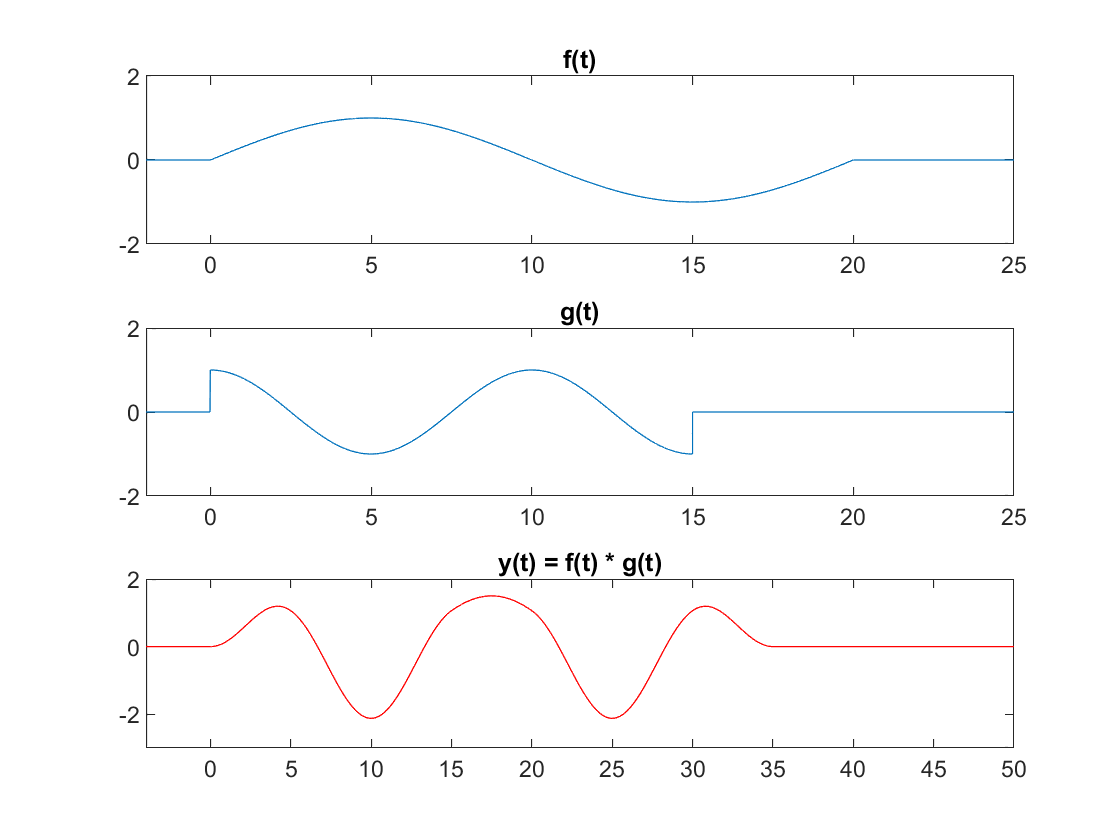
\includegraphics[width = 10cm]{plot3.png}
    \caption{\(f(t)\), \(g(t)\), and \(y(t)\)}
    \label{fig:thirdplot}
\end{figure}



\end{document}
